%\documentclass[a4paper,11pt,aas_macros]{report}

\documentclass[usenatbib]{mnras}
%Check if we are compiling under latex or pdflatex
% see e.g. http://www.2pi.info/latex/Includingeps.html
\ifx\pdftexversion\undefined \usepackage{epsf,epsfig}
%  \usepackage[dvips]{graphicx}
\else \usepackage[pdftex]{graphicx} \fi
\usepackage{lscape}
\usepackage{color}
\usepackage{amsmath}
%\usepackage{ulem}
\bibliographystyle{mnras}

%%%%%%%%%%%%%%%%%%%%%%%%%%%%
% ANY OTHER DECLARATIONS HERE:
\newcommand{\Herschel}{\textit{Herschel} }
\newcommand{\um}{\micron\  }
\newcommand{\STARFINDER}{{\sc starfinder}}
\newcommand{\DESPHOT}{{\sc desphot}}

%%%%%%%%%%%%%%%%%%%%%%%%%%%%


\title[HELP: The Herschel Extragalactic Legacy Project]{HELP: The Herschel
  Extragalactic Legacy Project\footnote{{\em Herschel} is an ESA space
  observatory with science instruments provided by European-led Principal
Investigator consortia and with important participation from NASA.}}
\date{June, 21st 2018}
\author[S. J. Oliver et al.]
{
  \parbox{\textwidth}
  {\raggedright S.J. Oliver$^{1}$\thanks{S.Oliver@Sussex.ac.uk},
  P.D.~Hurley,$^{1}$
  H.~Aussel,$^{7}$
  T.~Bakx,$^{20}$
  V.~Buat,$^{10}$
  D.~Burgarella,$^{10}$
  N.~Christopher,$^{35}$
  S.~Duivenvoorden,$^{1}$
  K.~Duncan,$^{30}$
  S.~Eales,$^{20}$
  A.~Efstathiou,$^{35}$
  E.A.~Gonz\'alez~Solares,$^{24}$
  M.~Griffin,$^{20}$
  M.~Jarvis,$^{40}$
%  E.~Le~Floc'h,$^{7}$
%  B.~Lo~Faro,$^{21}$
  V.~Papadopoulou,$^{35}$
  K.~Penner,$^{7}$
  E.~Rigby,$^{30}$
  H.~Rottgering,$^{30}$
  Y.~Roehlly,$^{1}$
  J.~Scudder,$^{1}$
  R.~Shirley,$^{1}$
  M.~Smith,$^{20}$
  M.~Vaccari,$^{40}$
  L.~Wang$^{2}$,
  E.~Pons$^{24}$,
  et. al.
}
\vspace{0.4cm}\\
\parbox{\textwidth}
{\raggedright
  $^{1}$Astronomy Centre, Dept. of Physics \& Astronomy, University of Sussex,
  Brighton, BN1 9QH, UK\\
  $^{7}$Laboratoire AIM-Paris-Saclay, CEA/DSM/Irfu - CNRS - Universit\'e Paris
  Diderot, CE-Saclay, pt courrier 131, F-91191 Gif-sur-Yvette, France\\
  $^{10}$Aix Marseille Univ, CNRS, LAM, Laboratoire d'Astrophysique de Marseille, 
Marseille, France\\
  $^{20}$School of Physics and Astronomy, Cardiff University, Queens Buildings,
  The Parade, Cardiff CF24 3AA, UK\\
  $^{24}$Institute of Astronomy, University of Cambridge, Madingley Road,
  Cambridge CB3 0HA, UK\\
  $^{2}$Netherlands Institute for Space Research, SRON\\
  $^{30}$Universiteit Leiden\\
  $^{35}$European University Cyprus\\
  $^{40}$UWC\\
  $^{50}$Stanford\\
}}

%%%%%%%%%%%%%%%%%%%%%%%%%%%%
% BEGIN DOCUMENT
\begin{document}
%\tableofcontents
\maketitle
%%%%%%%%%%%%%%%%%%%%%%%%%%%%


%%%%%%%%%%%%%%%%%%%%%%%%%%%%
\section*{Notes on draft}

{\color{red} This draft 21-June-2018 is a rough skeleton for comments by the
team.  Authorship is those who are funded participants, who contributed to the
proposal or have made an additional direct contribution to this paper. All
authors will be expected to provide comments or indicate that they are happy
with content. Authorship order is PI followed by Project Scientists and then
ordered  alphabetically, this may not be the final ordering, hence I've not
bothered sorting the institutional numbers. I was tempted to rip stuff out of
the proposal, but I think that might be too verbose. The table of contents is
obviously just to aid in understanding the structure}

\tableofcontents


\begin{abstract}
  We describe a new project to collate, curate, homogenise and add-value to most 
  of the premium multi-wavelength extragalactic data sets over 1300 ${\rm
  deg}^2$. The sky boundaries of \Herschel Extragalactic Legacy Project, HELP,  are currently defined by almost all of the \Herschel SPIRE extragalactic survey fields,
  notably the \Herschel Multi-tiered Extragalactic Survey (HerMES) and the
  \Herschel Atlas survey (H-ATLAS). HELP brings together data at all wavelengths
  from radio to X-ray.  This paper describes the motivation and the principle
  elements in the design of the project. Guiding principles are transparent or ``open" methodologies with care for reproducibility and identification of provenance. A Key element of the design focus
  around the homogenisation of calibration, meta data and the provision of
  information required to define the selection of the data in fashion that 
  they can be used for statistical analysis. This goes significantly beyond what is available in standard virtual observatory protocols. The full
  scientific exploitation of this requires novel methods.  We  advocate
  probabilistic methods that extract information directly from the maps at long
  wavelengths, exploiting the prior information available at shorter wavelengths
  and providing full sampling of the posteriors rather than traditional
  catalogues. 


  With this project definition paper we provide access to the first version of the full data set, and we provide a monolithic map of the largest SPIRE extragalactic
  field at 385 deg$^2$. We also provides some basic tools to access the
  information currently in the HELP database.   Software will made available
  through github.  The database, data, are available through ....
\end{abstract}

\begin{keywords}
  techniques: photometric -- catalogues -- surveys -- infrared: galaxies --
  submillimetre: galaxies -- galaxies: evolution
\end{keywords}
%-----------------------------------------------------
% Chapter
%-----------------------------------------------------
\section{Introduction}\label{sec:intro}


A fundamental requirement for rigorous testing of any theories of galaxy
formation and evolution is a complete statistical audit or census of the stellar
content and star formation rates of galaxies in the Universe at different times
and as a function of the mass of the dark matter halos that host them.

This audit requires many elements.   We need un-biased maps of large volumes of
the Universe made with telescopes that probe the different wavelengths at which
the different physical processes of interest manifest themselves. We need
catalogues of the galaxies contained within these maps with photometry estimated
uniformly from field-to-field, from telescope-to-telescope and from
wavelength-to-wavelength. We need to understand the probability of a galaxy of
given properties appearing in our data sets.  We need the machinery to bring
together these various data sets and calculate the ``value-added" physical data
of primary interest, e.g. the distances, stellar masses,
star-formation rates and the actual number densities of the different galaxy
populations.

For decades many  teams  have been undertaking ambitious coordinated
multi-wavelength programmes to study large volumes of the distant Universe.
These surveys are now becoming sufficiently complete that we are now able to
undertake the necessary homogenising and adding value and thus provide the first
representative and comprehensive census of the galaxy populations in the distant
Universe.

Collation of multi-wavelength data has been undertaken for very deep surveys
over small areas (less than few deg$^2$) in particular COSMOS\citep{cosmos} and ASTRODEEP\citep{astrodeep} and
for wide nearby surveys (over 200-1000 deg.$^2$) especially SDSS\citep{sdss} and GAMA\citep{gama}.
However, due to size of the data and complexity arising from the variety of
observatories required little concerted effort has been made to assemble the
deep surveys over 10-1000 deg.$^2$. These surveys are particularly important as
they are large enough to probe representative  ranges of environments and to
provide large statistical samples to  fully explore the range of galaxy
phenomena in detail and including rare, transitory phenomena.

ESA's {\em Herschel}\citep{pilbrat} mission has a unique role in these studies, probing the
obscured star-formation activity, which at high redshifts forms about 80\% of
all star formation The {\em Herschel} extra-galactic surveys were a major goal
of {\em Herschel} and occupied around 10\% of the {\em Herschel} mission.  These
surveys cover enough of the sky to provide representative samples of dark matter
halos including the most massive ones.

The {\em Herschel} SPIRE instrument is sufficiently sensitive that the maps can
detect most ($>60\%$) of the emission making up the cosmic infra-red background
radiation (CIBR), which itself makes up roughly half of the total background
radiation from galaxies.  However, the large beam size means that the objects
that can be clearly seen as individual sources only make up about 15\% of the
CIBR.  A particular focus of our HELP is to employ new methods to learn from our
large statistically meaningful samples the relationship between the ancillary
data  and the {\em Herschel} data and thus unlock the full information from the
{\em Herschel} maps and then make that available as a legacy to the community.

The final pieces of this multi-wavelength survey programme will be completed
with the optical, NIR and radio surveys being carried out during the lifetime of
this grant.  The VISTA near-infra-red surveys detect the radiation from the old
stellar population in galaxies, which accounts for most of the stellar mass,
while the radio surveys being carried out the next few years with LOFAR, MeerKAT
and ASKAP detect radiation associated with the young stellar population and with
AGN.

Statistical modelling of galaxy populations requires a detailed understanding
and modelling of the selection processes in the basic data products and the
derived properties.   These ``selection functions'' are seldom available for
individual data sets and rarely, if ever, published for derived physical
properties.  We will produce these and make them all public.

A key motivation of large area surveys is to probe galaxy populations in all
environments. Cluster catalogues and density maps are only really possible with
the homogeneous multi-wavelength data over wide fields we will have provided. So,
we will provide these to the community.

The techniques, tools and data we provide will enable astronomers in Europe to
fully capitalise on resources provided by {\em Herschel} and the other surveys,
extending the kinds of scientific investigation possible a decade ago in the
nearby Universe with the SDSS into the early Universe and providing a lasting
legacy for surveys and facilities in the future.  

This paper presents the HELP. In Section~\ref{sec:fields} we describe the define
the HELP fields.   In Section~\ref{sec:surveys} we describe . In
Section~\ref{sec:metrics} we provide metrics of the catalogue quality by
injecting synthetic sources.   In Section~\ref{HeLMSextended} we discuss
extended sources and artefacts. In Section~\ref{sec:catcomp} we compare with
similarly constructed catalogues of Herschel sources in the  HerS field
\cite{Viero:2014lr}, a 79 deg$^2$ field which has a 10 deg$^2$ overlap.  We
discuss the uses of this catalogue and future work in
Section~\ref{sec:discussion} and conclude in Section~\ref{sec:conclusions}.


\section{The HELP fields}\label{sec:fields}

Many extragalactic surveys from different observatories and different
wavelengths have been coordinated in their planning and execution. However, many
had different motivations and all had different factors constraining their
choice of field locations and sizes. So, to define a common boundary is
a challenge.  Nevertheless to collate a set of data we need to define some rigid
boundaries. Given that there is no imminent successor to  \Herschel  the data
from that mission provides a legacy benchmark.  Within the \Herschel observatory
the SPIRE instrument \citep{Griffin:2010lr} mapped larger areas than the PACS
instrument \citep{Poglitsch:2010lr}. We thus decided to define the boundaries of
the project on the basis of the extra-galactic surveys carried out with SPIRE.
The specific \Herschel OBSIDS chosen to define the project are listed in
Appendix~\ref{sec:obsids}

The \Herschel Multi-tiered Extragalactic Survey (HerMES, \citealt{Oliver:2012})
is a major survey conducted by the \Herschel mission\citep{Pilbratt:2010lr}
using the SPIRE \citep{Griffin:2010lr} and PACS \citep{Poglitsch:2010lr}
instruments.  The largest and shallowest of the HerMES SPIRE fields, making up
the bottom of the ``tiered wedding cake''  is the HerMES Large Mode Survey,
HeLMS.

\begin{table*}
  \begin{tabular}{|l|r|r|r|r|r|r|r|}
\hline
  \multicolumn{1}{|c|}{Name} &
  \multicolumn{1}{c|}{RA} &
  \multicolumn{1}{c|}{Dec} &
  \multicolumn{1}{c|}{RA min} &
  \multicolumn{1}{c|}{RA max} &
  \multicolumn{1}{c|}{Dec min} &
  \multicolumn{1}{c|}{Dec max} &
  \multicolumn{1}{c|}{Area} \\
  \multicolumn{1}{|c|}{} &
  \multicolumn{1}{c|}{[deg]} &
  \multicolumn{1}{c|}{[deg]} &
  \multicolumn{1}{c|}{[deg]} &
  \multicolumn{1}{c|}{[deg]} &
  \multicolumn{1}{c|}{[deg]} &
  \multicolumn{1}{c|}{[deg]} &
  \multicolumn{1}{c|}{[deg.$^2$]} \\
\hline
  SSDF & -8.1 & -55.1 & -357.8 & -18.5 & -60.5 & -48.5 & 110.4\\
  HATLAS-SGP & 1.5 & -32.7 & 337.2 & 26.9 & -35.6 & -24.5 & 294.6\\
  ELAIS-S1 & 8.8 & -43.6 & 6.4 & 11.2 & -45.5 & -41.6 & 9.0\\
  Herschel-Stripe-82 & 14.3 & 0.0 & 348.4 & 36.2 & -9.1 & 8.9 & 363.4\\
  XMM-LSS & 35.1 & -4.5 & 32.2 & 38.1 & -7.5 & -1.6 & 21.8\\
  CDFS-SWIRE & 53.1 & -28.2 & 50.8 & 55.4 & -30.4 & -26.0 & 13.0\\
  AKARI-SEP & 70.8 & -53.9 & 66.2 & 75.4 & -55.9 & -51.7 & 8.7\\
  GAMA-09 & 134.7 & 0.5 & 127.2 & 142.2 & -2.5 & 3.5 & 62.0\\
  COSMOS & 150.1 & 2.2 & 148.7 & 151.6 & 0.8 & 3.6 & 5.1\\
  Lockman-SWIRE & 161.2 & 58.1 & 154.8 & 167.7 & 55.0 & 60.8 & 22.4\\
  GAMA-12 & 179.8 & -0.5 & 172.3 & 187.3 & -3.5 & 2.5 & 62.7\\
  HDF-N & 189.2 & 62.2 & 188.1 & 190.4 & 61.8 & 62.7 & 0.67\\
  SA13 & 198.0 & 42.7 & 197.6 & 198.5 & 42.4 & 43.0 & 0.27\\
  HATLAS-NGP & 199.5 & 29.2 & 189.9 & 209.2 & 21.7 & 36.1 & 177.7\\
  XMM-13hr & 203.6 & 37.9 & 202.9 & 204.4 & 37.4 & 38.5 & 0.76\\
  EGS & 215.0 & 52.7 & 212.4 & 217.5 & 51.2 & 54.2 & 3.6\\
  GAMA-15 & 217.6 & 0.5 & 210.0 & 225.2 & -2.5 & 3.4 & 61.7\\
  Bo\"otes & 218.1 & 34.2 & 215.7 & 220.6 & 32.2 & 36.1 & 11.4\\
  ELAIS-N1 & 242.9 & 55.1 & 237.9 & 247.9 & 52.4 & 57.5 & 13.5\\
  ELAIS-N2 & 249.2 & 41.1 & 246.1 & 252.3 & 39.1 & 43.0 & 9.2\\
  xFLS & 259.0 & 59.4 & 255.6 & 262.5 & 57.9 & 60.8 & 7.4\\
  SPIRE-NEP & 265.0 & 69.0 & 263.7 & 266.4 & 68.6 & 69.4 & 0.6\\
  AKARI-NEP & 270.0 & 66.6 & 264.6 & 275.3 & 64.5 & 68.5 & 9.2\\
\hline\end{tabular}

  \caption{Summary of HELP fields.  The total area is 1269.1 deg.$^2$}
\end{table*}


\begin{figure*}
  \centering 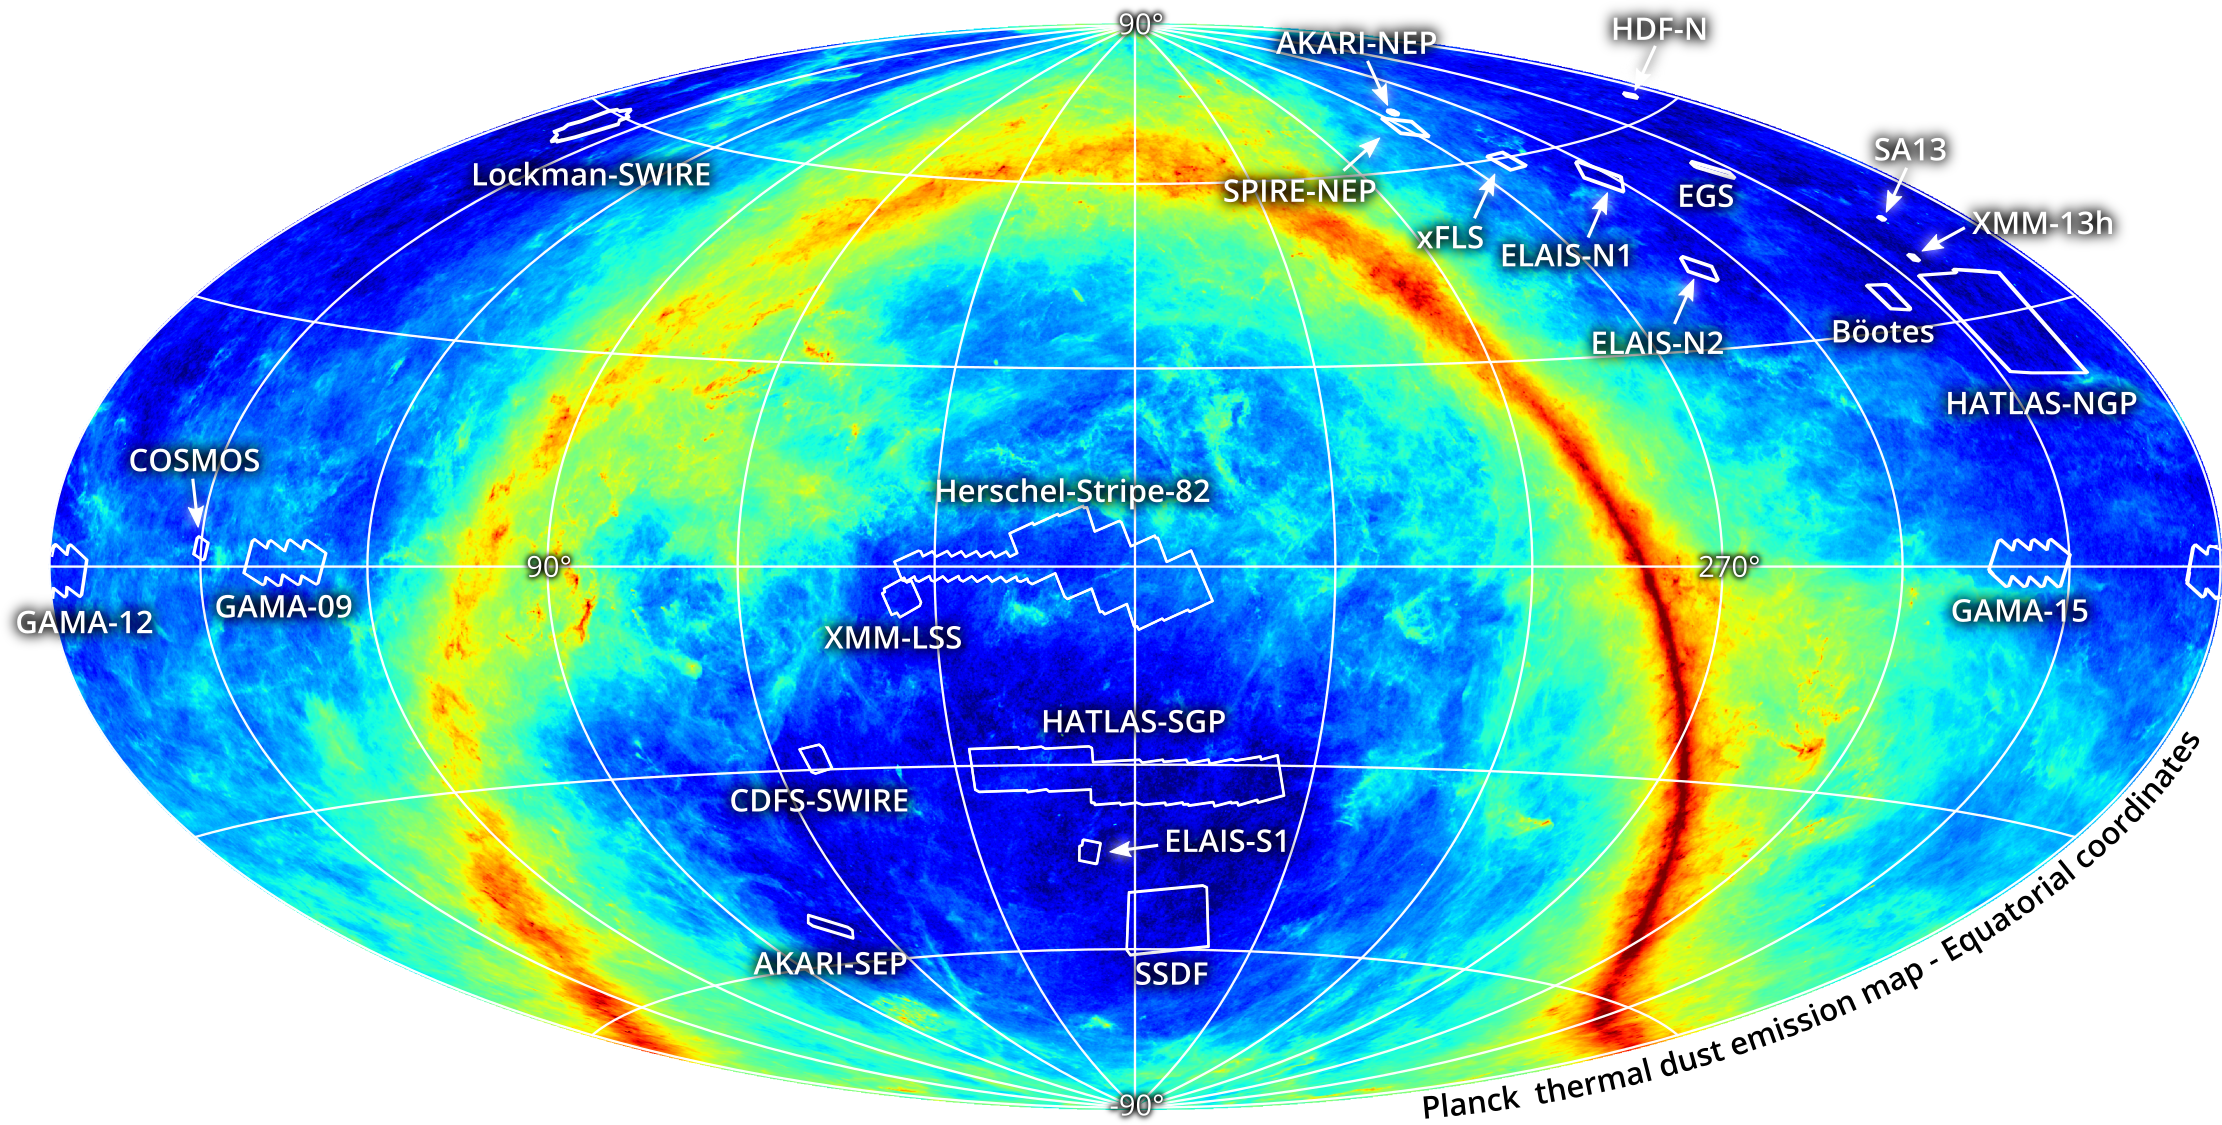
\includegraphics[width=16cm]{figs/HELP-fields.png}
  \caption[HELP Sky]{Projection of the HELP fields onto the dust emission from
    our own Galaxy.}\label{fig:helpsky}
\end{figure*}

\begin{figure}
  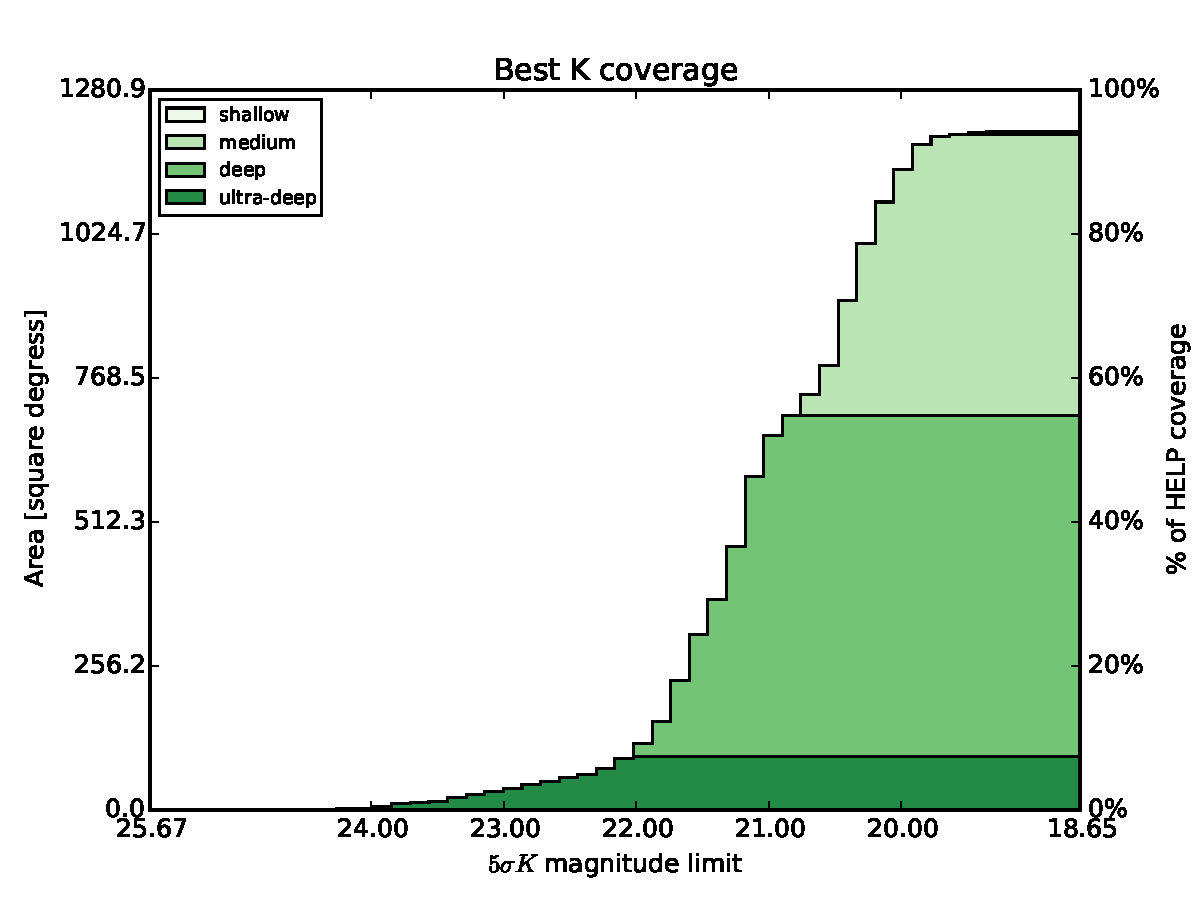
\includegraphics[width=8cm]{figs/K_coverage_v1_2_full.pdf}
  \caption[K-band coverage]{The cumulative area within HELP covered to a given
    $K_{\rm AB}$ depth. In this case the depth has been defined using the
    $\sigma$ from the flux errors of objects in the catalogues. This is an example
    of the summary report that can be generated from the HELP database. Similar
    plots can be generated for other bands, over individual fields and jointly
    limiting in more than one band. }\label{fig:k}
\end{figure}

\begin{figure*}
  \centering 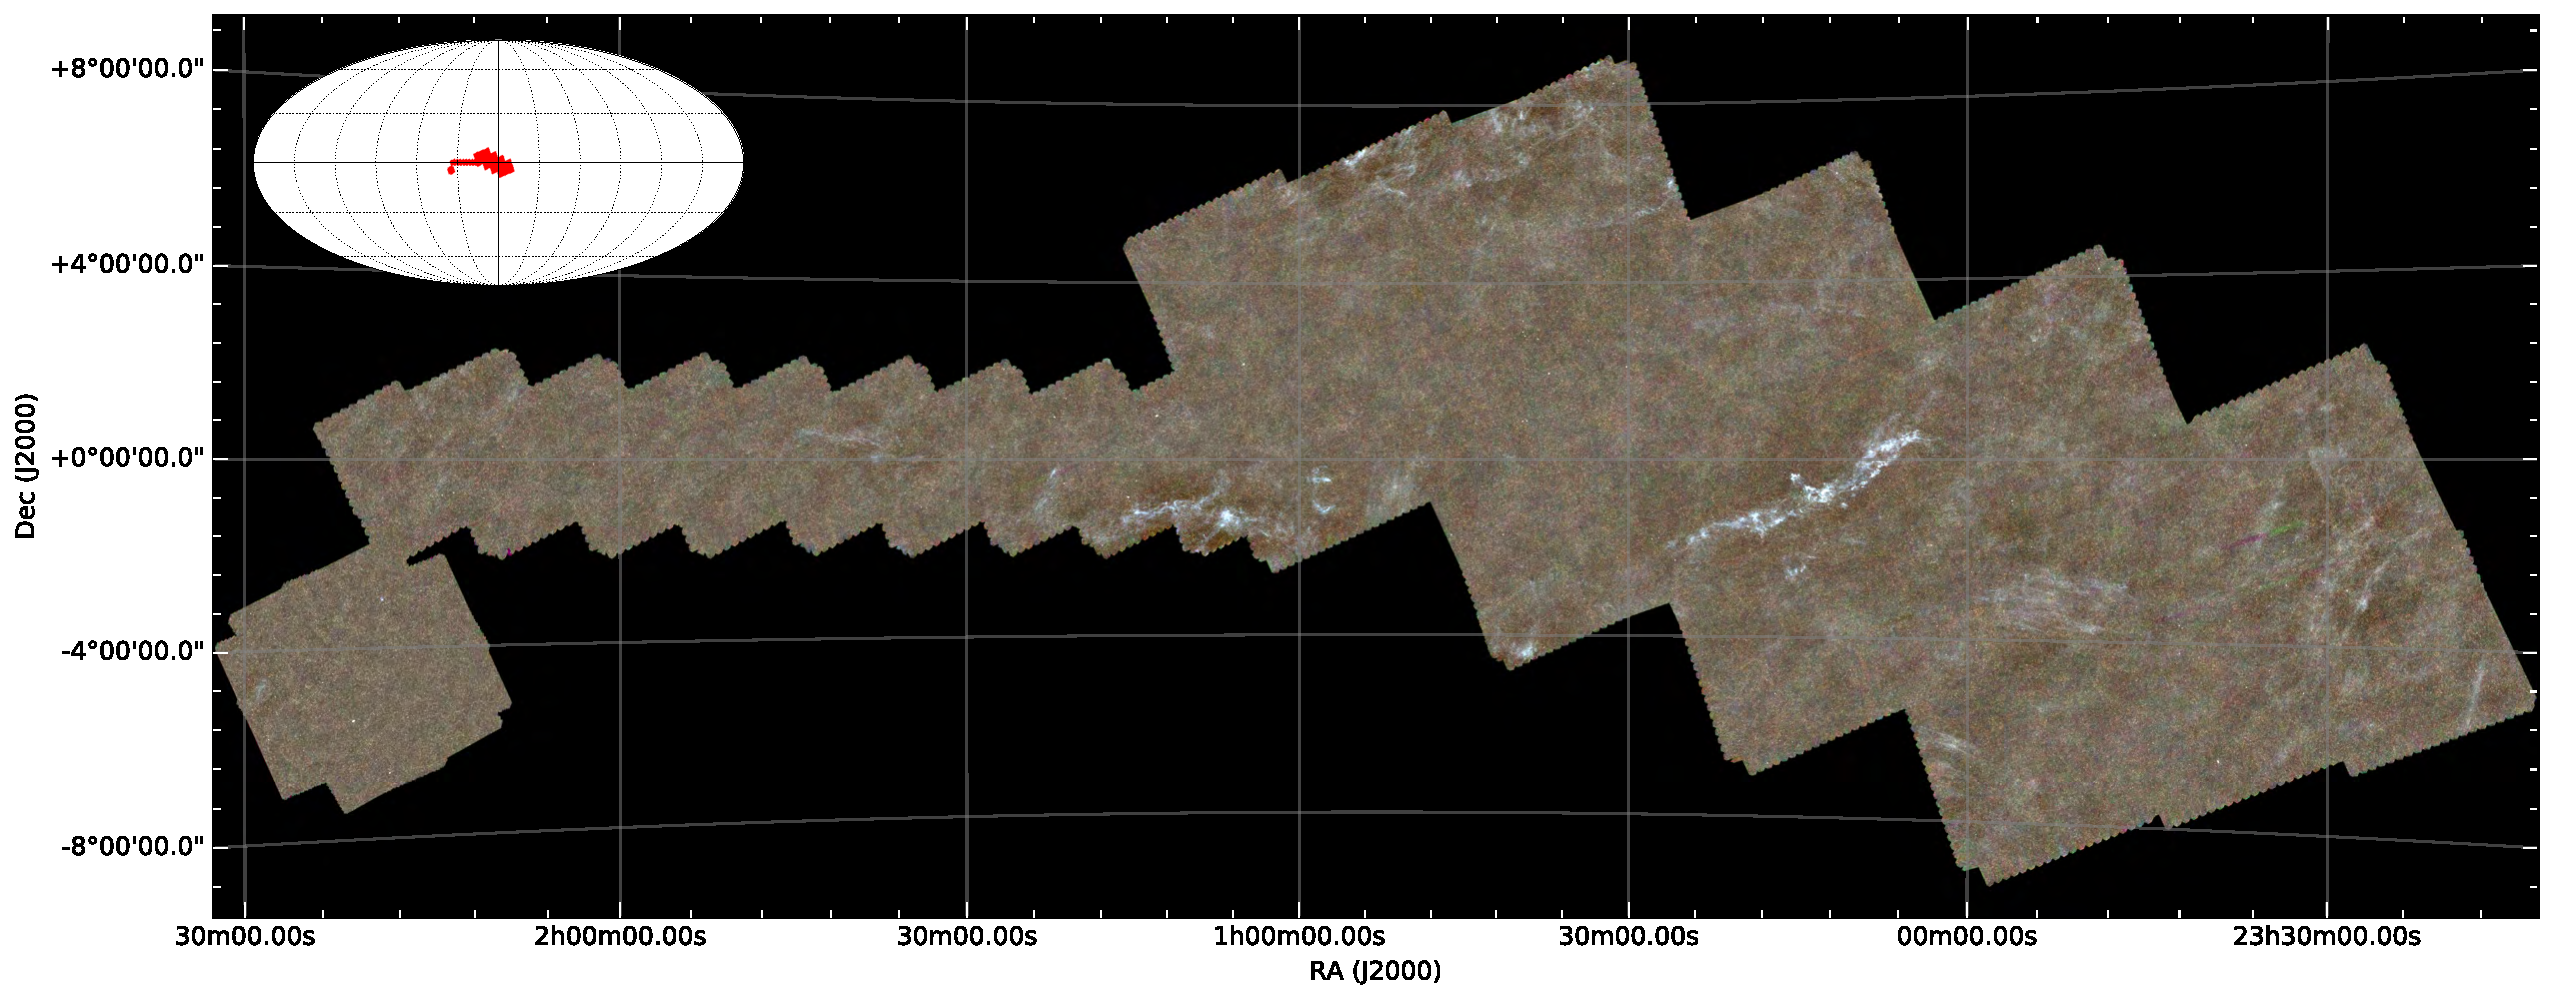
\includegraphics[width=16cm, angle=0]{figs/helms_hers_xmm-lss-rgb-sm.pdf}

  \caption[Three-colour image of Herschel Strip 82 region]{RGB representation of
    the Herschel Stripe 82 and XMM-LSS field, with 250\um, 350\um and 500\um
    represented by blue, green and red respectively. This is the largest
    contiguous extra-galactic region observed by \Herschel\.  The maximum scale
    of the field from the East to West tips is  50\degr and the separation from
    edge-to-edge (following the zig-zag, roughly North-to-South) is 11\degr. The
    inset indicates the location of this region on an all-sky equatorial
    projection. The total area of  this field is 385 deg.$^2$. Readily apparent
    is the strong cirrus structure throughout the map, including a ``seagull"
    like shape in the centre.  The data comes from three different observations
    (XMM-LSS, HELMS from HerMES \citealt{Oliver:2012} and the HERS. This maps
    was built for HELP from the processed SPIRE time-lines using the HerMES SMAP
    processing.}\label{fig:hs82}
\end{figure*}

\section{The multi-wavelength surveys}\label{sec:surveys}

\subsection{Data audit}
{\color{red} A Section to define the data that will be included}

\subsection{The depth of data}
{\color{red} A section to look at CIRB vs mag and the co-variances of the
multi-wavelength data }


\section{Data Curation}
\subsection{Homogenisation}
\subsection{Meta data}
\subsection{Selection Functions}
\begin{itemize}
  \item{Binary coverage:} Multi-Order Coverage maps, MOCs
  \item{Depth maps:} Multi-Order Depth maps, MODs
  \item{Completeness Curves:} Multi-Order Logistic Curves MOLCs. Based on
    logistic curve parameters, but also in multi-order
  \item{Full likelihood function:} Not quite sure what we mean here.
\end{itemize}


\section{The photometry work-flow}

{\color{red} A section to define the HELP pipeline.  }

In this section we describe the photometry work-flow.  We create a master list 
of astronomical sources and collate photometry measurements for these sources 
at all wavelengths. Part of this process involves determining the highest 
quality measurements available in a given field and wavelength region. In order 
for subsequent data processing to work effectively, there should be high quality 
photometry across a wide spread of wavelengths. This stage also allows us to 
investigate the depths available in a given area for a given band. Obviously,
some of the fields in the HELP areas have more high quality surveys available than others.
By using Jupyter notebooks to document all the processing on GitHub, all this 
information about data quality is readily available and the code could be rerun with future 
additional survey data. The forced photometry performed by XID+ takes the master list as a hard positional prior. This is then used to provide a further catalogue of far infra red flux measurements.

\subsection{Master list}
\label{sec:masterlist}
The HELP master list is contains optical, NIR and IRAC catalogues. It includes every 
source with a measurement in at least one band. A positional cross match is then
used to combine the various wavelengths and all sources are flagged to specify
which regions it has measurements as well as whether it was in an area covered by a
given band. Therefore if the object was not detected in some band and we have a measure 
of the depth available in that band, we have a measure for an upper limit for the flux in
that band. We also provide a table of the original catalogue ids and the original catalogues.
This means that where additional useful information is included in the input catalogue,
it can be quickly recovered using the table of cross identifiers. All this data is provided in a
simple and well documented structure to facilitate independent validation and external use.
{\color{red} outline of the work-flow to (a) define the master list, (b) reject
spurious sources including artefacts and those around bright stars stars (c)
classification of sources }

the master list for each field will have different levels of sophistication.

\begin{itemize}
  \item{Baseline: point list}
  \item{Silver: point list, with size and shape}
  \item{Gold: two component shape model (bulge and disk)}
  \item{Platinum: full morphological description e.g. based directly on
    short-wavelength image}
\end{itemize}

\subsection{Forced photometry}

With high resolution data we will provide photometry either by matching
catalogues or by returning to the images and extracting the photometry if the
original catalogues do not include the photometric data we require.

\subsection{A prior model}
\begin{itemize}
  \item{positional priors}
  \item{flux priors}
  \item{observed colour priors}
  \item{redshift, SED priors}
  \item{luminosity/environment priors}
\end {itemize}

\subsection{\emph{XID+}: the probabilistic deblender for confusion dominated maps}
For many of our fields, in addition to the SPIRE maps we also have Spitzer MIPS $\mathrm{\mu m}$ and Herschel PACS 100 and 160 $\mathrm{\mu m}$ maps that cover the mid to far-infra-red part of the electromagnetic spectrum. However, due to the relatively large beam size of the these maps compared to the galaxy density (≈30 per SPIRE beam for optical sources with B < 28), multiple galaxies can be located within the instrument beam. This is referred to as the problem of source confusion.

To obtain accurate photometry from these infra-red maps, overcoming the source confusion problem is essential. One way to solve the problem is to use prior information to accurately distribute the flux in the maps to the underlying astronomical objects. For example, if we know the location of a galaxy to a reasonable tolerance (e.g. from an optical image where resolution is better), we may expect a galaxy to be found in the MIPS, PACS and SPIRE maps at the same location.

As part of HELP, we have developed \emph{XID+} \citep{Hurley:2017} which uses a probabilistic Bayesian approach that provides a natural framework in which to include prior information and obtain the full posterior probability distribution on flux estimates. Obtaining the full posterior probability distribution is particularly important for getting accurate uncertainties on source flux.

\subsubsection{HELP XID+ pipeline}
HELP uses XID+ to carry out forced photometry on the Spitzer MIPS, Herschel PACS and Herschel SPIRE maps. As the output fluxes are products for the main database, we stick to positional and uninformative flux priors (i.e. uniform flux prior) to enable the widest range of analysis with the HELP data products. Additional prior information is a powerful approach to get more out of the data, however their use must be fully understood and taken into account when carrying out further analysis. For example, the fluxes coming from a version of XID+ that uses SED templates as a prior, cannot then be used to fit SEDs with a different set of templates. We have explored numerous ways of adding additional prior information and provide these as part of the XID+ software package for users to carry out their own sophisticated fitting on their chosen sources. 

Our list of prior sources are constructed from the master list, described in Section \ref{sec:masterlist}. Ideally, we would use all sources in the master list as our prior list. In reality, there are too many sources to constrain from the data, unless one goes to more informative priors. We therefore cut down the master list to sources detected in bands that are good tracers of infrared emission, such as K band or IRAC \citep{Duivenvorden:2018}. For fields covered by Spitzer, we use sources detected in any of the Spitzer IRAC bands. To remove any possible artefacts in the IRAC catalogues, We impose an additional constraint that sources must also have a detection in either the optical or NIR wavelength range (using the $opt_nir_det$ flag). 


%IRAC prior, selection function, opt_nir_detection, MIPS detection, notebooks
%flag
\subsubsection{HELP XID+ data products}
\subsubsection{XID+ extensions}

%reason for full prob dist. e.g. DESPHOT
%: Pipeline for HELP: explanation for not going beyond positional priors
%Products: marginalised catalogues, Bayesian P-value maps, software to re run and obtain full posterior 
%Additional extensions: CIGALE, full SED

\subsection{Blind catalogues, cross-matching and supplementary lists}

An essential step in achieving the latter goals and for providing a legacy data
set, suitable for community exploitation is to construct a catalogue of objects
detected in the SPIRE maps without reference to any other data and with fluxes
extracted at the SPIRE wavelengths (a `blind" catalogue).  These catalogues give
a perspective of the sub-mm sky unaffected by any prior prejudice. One
significant challenge is the large SPIRE beam, leading to source confusion (e.g.
\citealt{Nguyen:2010lr}) which requires careful de-blending and the resultant
catalogues of sources do not necessarily correspond one-to-one to individual
galaxies.   To enable statistical studies key metrics for these catalogues are
required to assess: positional and flux biases and accuracy; completeness and
reliability.   Similar catalogues and metrics have been produced and made public
for the other HerMES fields \citep{Smith:2012lr,Wang:2013lr}. A particular
challenge for HeLMS is the high level of emission (``cirrus") from our own
Galaxy.

\section{Added value}

\subsection{Photometric redshifts}

\subsection{Physical modelling}

\section{Tools}

The philosophy with HELP is that we should be providing the data, meta data and
tools that astronomers can easily carry out their scientific investigations
without a high level of instrument or survey-level expertise.  We have defined
some specific scientific use-cases which should be achievable at the end of the
project.  These are aimed to result in recipes at the level  that a postgraduate
student (under the supervision of an astronomer) could take and produce
meaningful scientific results.  Our intention is that all scientific results
from the team could be easily reproduced using these tools.  We anticipate that
some of these tools will be database operations.  Our database is VO enabled
with ADQL interfaces.  Some tools will be traditional client/server interfaces.
Other tools will be developed to provide containers (e.g. Docker) that the user
can down-load and run on their own CPU resources.  All software will be made
open source and distributed through public repositories (e.g. GIThub).

\section{Discussion and Conclusion}

%%%%%%%%%%%%%%%%%%%%%%%%%%%%
% BIBLIOGRAPHY


\section*{Data used in this paper}

The catalogue described in this paper is available at \url{hedam.lam.fr/HerMES}

HELP comprises the  Herschel OBSIDS: 1342257362, 1342247216,
1342246632, 1342246580, 1342238251, 1342237563, 1342237553, 1342237550,
1342236240, 1342236234,1342236232, 1342234749.

All products available through the HELP www pages \url{herschel.sussex.ac.uk}.




\section*{Acknowledgements}

%Charlotte Clarke acknowledges support from the Science and Technology
%Facilities Council (grant number ST/J50077X/1)

The research leading to these results has received funding from the European
Union Seventh Framework Programme FP7/2007-2013/ under grant agreement No.
607254.


Seb Oliver acknowledges support from the Science and Technology Facilities
Council (grant number ST/L000652/1)


HCSS / HSpot / HIPE are joint developments by the Herschel Science Ground
Segment Consortium, consisting of ESA, the NASA Herschel Science Center, and the
HIFI, PACS and SPIRE consortia.

This research has found TOPCAT \citep{2005ASPC..347...29T} extremely useful.

This research has made use of the NASA/IPAC Extragalactic Database (NED) which
is operated by the Jet Propulsion Laboratory, California Institute of
Technology, under contract with the National Aeronautics and Space
Administration.

SPIRE has been developed by a consortium of institutes led by Cardiff Univ. (UK)
and including Univ. Lethbridge (Canada); NAOC (China); CEA, LAM (France); IFSI,
Univ. Padua (Italy); IAC (Spain); Stockholm Observatory (Sweden); Imperial
College London, RAL, UCL-MSSL, UKATC, Univ. Sussex (UK); Caltech, JPL, NHSC,
Univ. Colorado (USA). This development has been supported by national funding
agencies: CSA (Canada); NAOC (China); CEA, CNES, CNRS (France); ASI (Italy);
MCINN (Spain); SNSB (Sweden); STFC, UKSA (UK); and NASA (USA).

HELP would like to thank the HELP Scientific Advisory Board members past and
present for invaluable advice in the defining of the project: Simon Driver,
Loretta Dunne, Carol Lonsdale, Mark Lacy, Peter Capak, Takashi Onaka, Mara
Salvato, Brent Groves, G\"{o}ran Pilbratt, David Elbaz

Huge thanks also to our Project Manager, Louise Winters, for keeping us on-track
and on-time with good humour.

The data presented in this paper is released through the {\em Herschel} Database
in Marseille HeDaM ({\url{http://hedam.lam.fr/HerMES}})

\bibliography{./HELP_bib}

%%%%%%%%%%%%%%%%%%%%%%%%%%%%


%%%%%%%%%%%%%%%%%%%%%%%%%%%%
% START APPENDICES
\appendix


% \section{HeDAM standards}\label{sec:standards}

% Only needed if we are going to publish these, maybe even they are obsolete now?

\section{Multi-wavelength Survey Audit}

In this section we briefly summarise the data that is anticipated to be included
in HELP.   The summaries are grouped into broad wavelength regions over which
the properties are similar. We also highlight any specific value that HELP
expects to add to these data.

\subsection{X-ray}

\subsection{UV}

\subsection{Optical}

\subsection{NIR: 1-3\micron}

The whole of HELP is of course covered by the 2MASS survey and this data set
provides us with a key astrometric reference and a homogeneous catalogue of
sizes.  In the  near infrared the primary data products that are available are
the UKIRT and VISTA public surveys.  These overlap with most of the survey
fields. A few of the fields are substantially better covered by other surveys.
In Table~\ref{tab:k} we summarise the specific surveys that are currently
expected to be included in HELP.  Using our depth maps (see e.g.
Figure~\ref{fig:k}) we have also estimated the area in deg.$^2$ that are covered
above a few (arbitrary) $K_{\rm AB}$ limits to give some idea of the coverage.

These wavebands form a primary source for our master lists and thus drive the
selection functions.

The key value that will be added by HELP at these wavelengths is consistent
photometry extracted where necessary from the original survey images.

% \begin{table*}
%   \begin{tabular}{|l|r|r|l|r|r|r|r|l|}
\hline
  \multicolumn{1}{|c|}{Name} &
  \multicolumn{1}{c|}{RA} &
  \multicolumn{1}{c|}{Dec} &
  \multicolumn{1}{c|}{Key Data} &
  \multicolumn{1}{c|}{$K_{\rm AB}>23.7$} &
  \multicolumn{1}{c|}{$K_{\rm AB}>22$} &
  \multicolumn{1}{c|}{$K_{\rm AB}>20.75$} &
  \multicolumn{1}{c|}{$K_{\rm AB}>19.5$} &
  \\
\hline
  SSDF & -8.1 & -55.114 & VISTA-VHS &  & 9.7 & 45.0 & 105.0 & \\
  HATLAS-SGP & 1.5 & -32.734 & VISTA-VHS &  & 7.3 & 292.0 & 294.0 & \\
  ELAIS-S1 & 8.8 & -43.585 & VISTA-VIDEO & 2.8 & 2.8 & 3.4 & 8.9 & \\
  Herschel-Stripe-82 & 14.3 & -0.034 & VISTA-VHS &  & 7.5 & 86.2 & 374.0 & \\
  XMM-LSS & 35.1 & -4.528 & VISTA-VIDEO & 1.0 & 10.5 & 13.2 & 21.5 & \\
  CDFS-SWIRE & 53.1 & -28.235 & VISTA-VIDEO & 2.6 & 4.6 & 8.7 & 12.0 & \\
  AKARI-SEP & 70.8 & -53.862 & VISTA-VHS &  &  & 1.7 & 7.3 & \\
  GAMA-09 & 134.7 & 0.513 & VISTA-VIKING &  & 0.4 & 56.2 & 61.2 & \\
  COSMOS & 150.1 & 2.218 & VISTA-ULTRAVISTA & 1.0 & 1.0 & 1.2 & 5.0 & \\
  Lockman-SWIRE & 161.2 & 58.058 & UKIDS-DXS &  & 10.4 & 10.5 & 10.8 & \\
  GAMA-12 & 179.8 & -0.482 & VISTA-VIKING &  & 3.1 & 59.0 & 61.9 & \\
  HDF-N & 189.2 & 62.241 & Various &  &  &  &  & \\
  SA13 & 198.0 & 42.715 & ? & 0.2 & 0.2 & 0.2 & 0.2 & \\
  HATLAS-NGP & 199.5 & 29.215 & UKIDS-LAS &  & 18.1 & 62.1 & 179.0 & \\
  XMM-13hr & 203.6 & 37.918 & ? &  & 0.7 & 0.7 & 0.7 & \\
  EGS & 215.0 & 52.72 & ? &  & 0.1 & 0.7 & 0.7 & \\
  GAMA-15 & 217.6 & 0.456 & VISTA-VIKING &  & 1.2 & 60.2 & 60.9 & \\
  Bo\"otes & 218.1 & 34.173 &  &  & 4.9 & 5.2 & 5.2 & \\
  ELAIS-N1 & 242.9 & 55.071 & UKIDS-DXS &  & 9.4 & 9.8 & 9.9 & \\
  ELAIS-N2 & 249.2 & 41.058 & UKIDS-LAS &  & 0.1 & 0.2 & 0.8 & \\
  xFLS & 259.0 & 59.384 & UKIDS-LAS &  & 0.1 & 2.6 & 2.7 & \\
  SPIRE-NEP & 265.0 & 69.004 & UKIDS-LAS &  &  &  &  & \\
  AKARI-NEP & 270.0 & 66.556 & UKIDS-LAS &  &  &  &  & \\
  Total	&	&	&	& 7.6	&92.1	&718.8	&1221.7\\
\hline\end{tabular}

%   \caption{Audit of data in near infra-red bands}\label{tab:k}
% \end{table*}

% \subsection{Mid-IR: 3.6-12\micron}

% \subsection{FIR: 24-500\micron}

% \subsection{sub-mm}

% \subsection{Radio}

% \subsection{Spectroscopic Redshifts}

\section{OBSIDS}

This Appendix lists the OBSIDS used in HELP

%%%%%%%%%%%%%%%%%%%%%%%%%%%%

%%%%%%%%%%%%%%%%%%%%%%%%%%%%
% END DOCUMENT
\end{document}
%%%%%%%%%%%%%%%%%%%%%%%%%%%%
